%!TEX root=../thesis.tex
\chapter{A Real-Time model for WebGL} \label{cha:rt_model}

WebGL is a relatively new technology that enables hardware-accelerated web
contents. Moreover, in the last few years Virtual Reality (VR) has became
another very popular research topic. The Mozilla Foundation is actively working
for bringing VR technologies to the web by means of WebVR~\cite{mozvr}. WebVR is
``an open specification that makes it possible to experience VR'' inside a web
browser, whose main goal is to make VR experiences easier, regardless of the
device used. This specification~\cite{webvrspecs} is available
via different frameworks like Mozilla's A-Frame~\cite{aframe}, which allows
to build virtual reality scenes inside the browser using only HTML and JavaScript
code.\\
This may seem a very different field with respect to the one of this
thesis, but what makes A-Frame similar to Cesium is how they exploit WebGL to
interact with the GPU to achieve hardware acceleration. In this sense it is
reasonable to compare VR and 3D-maps web technologies since they both use WebGL
in their core. Furthermore, virtual reality applications are even more
performance-demanding from the real-time point of view, since even relatively
small latencies (ie. in the order of tenths of milliseconds) can make a product
completely unusable and annoy the human eyesight.


\section{Assumptions} \label{sec:assumptions}
First of all, all the experiments presented in this thesis are run on a Dell
Inspiron 15R 5521 notebook\footnote{\url{http://www.dell.com/us/dfh/p/inspiron-15r-5521/pd}.},
whose hardware specifications are shown in Table \ref{tab:notebook_specs}.
Since 3D graphics performance highly depends on the GPU installed on the system,
the results presented in Chapter \ref{cha:experiments} are likely to be overtaken
if better graphics hardware (eg. a more powerful dedicated GPU) is installed.
\begin{table}[!htb]
    \centering
    \caption{The test machine hardware specifications.}
    \label{tab:notebook_specs}
    \begin{tabular}{|l|l|l|l|}
    \hline
    \multicolumn{1}{|l|}{\textbf{CPU}} & \multicolumn{1}{l|}{\textbf{GPU (integrated)}} & \multicolumn{1}{l|}{\textbf{RAM}} & \multicolumn{1}{l|}{\textbf{Hard drive}} \\ \hline
    Intel i7 3537U & Intel® HD Graphics 4000 & 8GB DDR3 & Samsung 850 Evo 250GB \\ \hline
    \end{tabular}
\end{table}

Another important aspect is how tests are conceived. As it is always the case in
real-time analysis, the worst possible scenario is the one of interest for
computing the WCET of a task. To achieve this situation in the test application,
Google Chrome is always run from scratch with only one active tab. Moreover, the browser
is forced not to cache any part of the JavaScript application code but,
at the same time, it is essential to eliminate the map retrival time.
Usually map tiles are
downloaded via HTTP using the REST APIs a terrain server exposes to the clients.
Even the time the navigator takes to download a small portion of the terrain
can be orders of magniture bigger than all the rest of the response/computation time.
Hence, this objective is obtained allowing the browser to locally save the
tiles downloaded during a ``warm-up'' phase. This allows to significantly lower
the map retrival time during the ``real'' experiment without jeopardizing the
timings of the entire trace.

Finally, picking timestamps during the execution of a piece of software can bias
the correctness of the data. This is another point that has to be
taken into account during any type of analysis involving time measurements like
the one presented in this work. In simple terms, measuring time takes time and
it does not come for free.


\section{Tools used}
This section presents the tools used to profile the test application and to pick
the timings needed for the experiments shown in Chapter \ref{cha:experiments}.
Even though the description reflects the specific usage in this work, these
software toolkits can be applied to a wide variety of fields and scenarios.

\subsection{Web Tracing Framework} \label{sec:wtf}
The Web Tracing Framwork (WTF)~\cite{wtf} is composed of a set of tools for
instrumenting, analyzing and visualizing web application execution traces.
It is an extensible framework able to capture and to replay HTML5 canvas elements
along with its WebGL content. In this way it is possible to implement a plugin for
this framework that is specific for the purpose of the application under test.
Furthermore, a wide set
of methods and events can be tracked out-of-the-box for preliminar investigations.

WTF is a very good toolset for an high-level analysis of web applications,
providing easy code instrumentation to track only what is truly interesting for the developer.
The usual work-flow is the following. First the events to be traced 
are selected, either from a predefined set or specific code instrumentation can be
inserted inside the source code using the framework's APIs. After that, the application's source code
has to include four the proper function calls to control the tracing mechanism.
An example of application source code is the following:
\begin{lstlisting}[caption=Usage example of the Web Tracing Framework., language=JavaScript,
  label=code:wtf_example]
  let wtfOptions = { ... }; // customize WTF behaviour
  wtf.trace.prepare(wtfOptions);
  /* application initialization */
  wtf.trace.start(); // start profiling
  /* code to be traced goes here */
  wtf.trace.snapshot("file://trace"); // save trace to file
  wtf.trace.stop(); // stop profiling
\end{lstlisting}

After taking a snapshot of the current trace (line 6, code snippet \ref{code:wtf_example})
and stopping capturing data (line 7), the trace is exported in a
compressed format that can be manipulated using some CLI
scripts\footnote{\url{https://github.com/google/tracing-framework}.} to export
data in Comma Separated Values (CSV) format. Otherwise the results can be visualized
thanks to the proper web
page\footnote{\url{http://google.github.io/tracing-framework/bin/app/maindisplay.html}.}.

Another highlight is its extendibility. In this way the developer can either
profile the application using the default events emitted by the browser or can 
directly instrument the source code to track only very specific parts. Basically, this
allows to measure nearly everything that is accessible from JavaScript, even
though it may not be enough in some situation.

Finally, a post-process task is required to get insights from the raw data.
The CSV exported by the Web Tracing Framweork has the following structure:
\begin{equation*}
    <time,\,value,\,total\_time,\,own\_time,\,arguments>
\end{equation*}

where:
\begin{itemize}
    \item \emph{time}: it is the amount of time (in milliseconds) elapsed from the
        \emph{wtf.trace.start()} function call.
    \item \emph{value}: it is the function name that is traces. More specifically this
        value is a string composed by\\
        ''\([context\_name]\#[function\_name]\)''.
    \item \emph{total\_time}: it is the time taken to complete the current invocation
        of the function (in milliseconds) along with any other function that
        is called.
    \item \emph{own\_time}: it is how long it took to complete the current invocation
        of the function (in milliseconds) without including any function called by
        the current one.
    \item \emph{arguments}: they all the arguments (with values) that are passed
        to the \emph{value} function.
\end{itemize}

Clearly, being the computaton of latencies the main aim this framework, the most
relevant fields to be later analyzed are the \emph{time}, the \emph{total\_time}
and the \emph{own\_time} values.


\subsection{Chrome's trace event profiler}
The other foundamental tool used to trace the test application is the trace
event profiler embedded into Google Chrome. This is another important reason why
Chrome is preferred as browser for the entire work, since it allows to diagnose
performance issues and to see what Chrome is really doing ``under the surface''.
This tool is available by default in any build of Google Chrome typing
\emph{chrome://tracing} inside the main URL bar.

This profiler ``records all the C++ and JavaScript method signatures in a
hierarchical view for each thread in each process'' of the browser. This results
in a huge amount of information, but it helps to identify performance bottlenecks
and to spot any kind of event happening to the browser instance. Hence, this tool
allows to
better analyze a web application, collecting all the events occuring when the
application is running starting from the renderer processes IPC up to every single
function that is executed by the GPU process.

Sometimes it may be necessary
to run Chrome with some particular command line flag in order to enable the
``debugging mode'' for some feature. For example, the \emph{--enable-skia-benchmarking}
flag is needed for profiling the Skia graphics engine. These additional flags
are not used by default since users do not need to profile the entire browser
all the time and thus, skipping some instruction inside the browser's source code
can result in better response times and navigation fluency.

Consequently, it is possible
to say that this event profiler perfectly fits a low-level analysis of everything
that happens inside the complex architechture of Google Chrome.
As it is possible to see from Figure \ref{img:chrome_event_profiler}, this tool
is capable not only to acquire data from the browser but also to visualize them
as flame graphs~\cite{gregg2016flame}.
\begin{figure}[!htb]
    \center{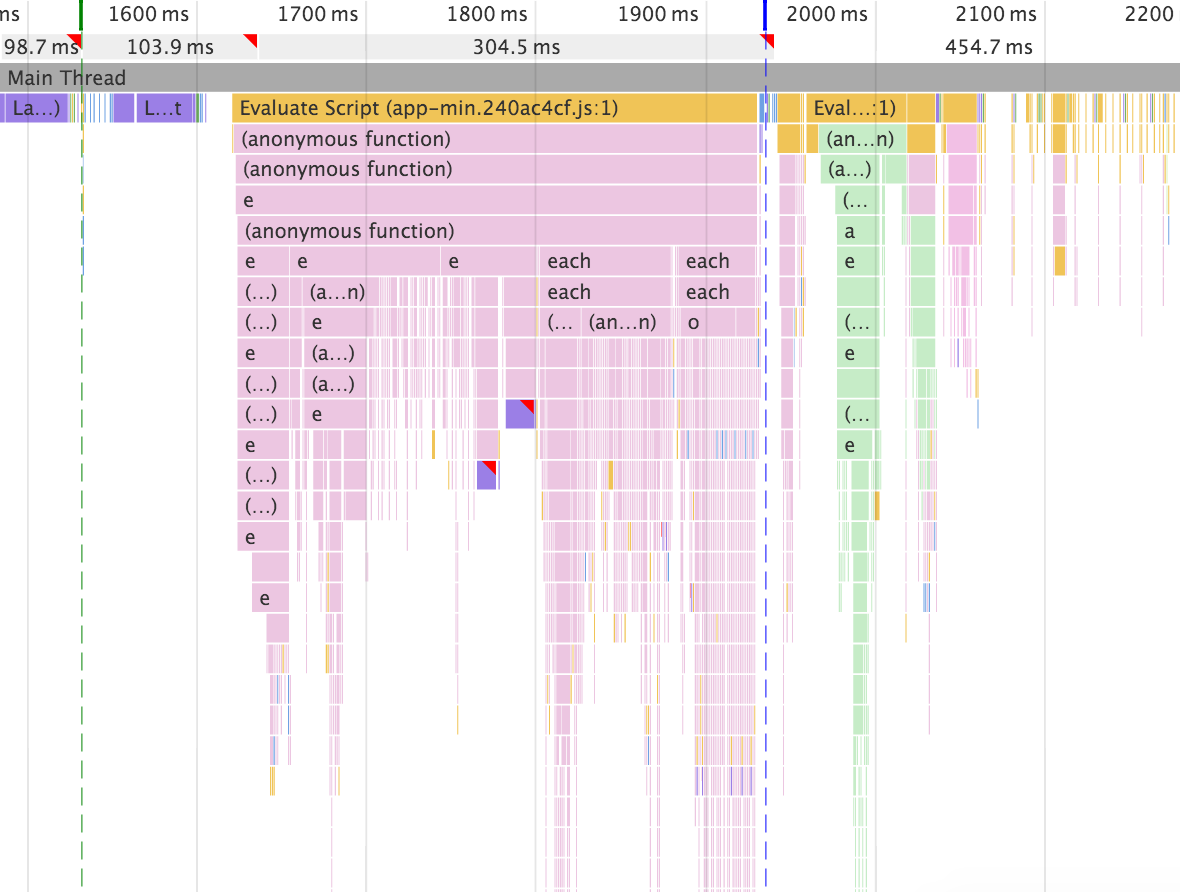
\includegraphics[width=0.47\linewidth]{chrome_event_profiler.png}}
    \caption{The viewer user interface for the Chrome event profiler.}
    \label{img:chrome_event_profiler}
\end{figure}

The output format of this tool is a JavaScript Object Notation (JSON) file with
several fieds. The ones of interest for the purpose of this work are the following:
\begin{lstlisting}
{
  "pid": 5782,
  "tid": 5782,
  "ts": 3951728304,
  "ph": "X",
  "cat": "gpu",
  "name": "GpuCommandBufferStub::OnAsyncFlush",
  "args": { ... },
  "dur": 113,
  "tdur": 112,
  "tts": 1213475
}
\end{lstlisting}

where:
\begin{itemize}
    \item \emph{pid}: it is the process id of the process outputting the event.
    \item \emph{tid}: it is the thread id for the thread outputting the event.
    \item \emph{ts}: it is the tracing clock timestamp (in microseconds), meaning
        the amount of time elapsed from the tracing start.
    \item \emph{ph}: it is the event type that is recorded. This is a single character
        that depends on the type of event being tracked\footnote{A complete list
        of the type of events available can be found at the following link:
        \url{https://docs.google.com/document/d/1CvAClvFfyA5R-PhYUmn5OOQtYMH4h6I0nSsKchNAySU/}.}
    \item \emph{cat}: it represents the event category. This a list used to hide
        events from the Trace Viewer user interface.
    \item \emph{name}: it is the name of the event.
    \item \emph{args}: this contains any argument that is provided to the event/function
        call.
    \item \emph{dur}: it specifies the tracing clock duration of complete events
        (in microseconds).
    \item \emph{tdur}: it specifies the thread clock duration of complete events
        (in microseconds).
    \item \emph{tts}: it specifies the thread clock timestamp of the event (in
        microseconds).
\end{itemize}

Among all the abovementioned values, the most important ones during the experiments
are the \emph{ts} and the \emph{tdur}; they allow to specify when an event has been
fired and for how much time the thread computing that function run.


\section{Profiling and analysis procedures} \label{sec:procedure}
Some extra work has been done to provide a very convenient way
for capturing data with the tool presented in the previous section. A program
simulating the FriWalk hardware has been developed to send the values for position
and rotation to the web
interface via the WebSocket protocol. This is useful to emulate the behaviour of
a portion of the system architechture (see Figure \ref{img:system_arch}) that was
not always available during the development of this thesis.

Even from the very first test with WTF it became clear that the system under
test is as complex as the problem this thesis aims to solve. Therefore, the hard
problem of profiling the entire navigator application is split into many simpler
parts. Moreover, the navigator is traced from its startup until the first new
position is sent by the FriWalk and it is displayed on the screen. This idea of reducing the
amount of workload to the minimum allows to better concentrate on fewer and more
specific data outputted by the two tracing tools. Hence, four different scenarios
have been implemented:
\begin{itemize}
    \item the complete navigator application.
    \item a ``camera-only'' mode; in this scenario there is no physical placeholder
        to be moved on the map and only the user's camera is moved.
    \item a ``no-map'' mode; in this scenario the map is completely
        excluded from the application, meaning that no tail for the terrain is
        downloaded.
    \item a ``redraw'' mode; this is a scenario simulating a walker that remains
        always stationary in the same position.
\end{itemize}

All the scenarios mentioned above aims at simplifying the post-processing
analysis and to focus on the different parts of the navigator. For example, the
``no-map'' mode is conceived to get rid of the map but, at the same time, to keep
all the base functionalities of the navigator. To some extent, the partial traces
obtained from all these scenarios can be utilized to compare each other and spot
their similarities and/or differencies.

Finally, a Python script is used to split and to graphically display the
timings extracted from the traces. Having a visual representation is often very
useful to better undestand what is happening as the time passes inside the application
trace.
